% Created 2021-09-03 Fri 09:02
% Intended LaTeX compiler: pdflatex
\documentclass{article}
\usepackage[utf8]{inputenc}
\usepackage[T1]{fontenc}
\usepackage{graphicx}
\usepackage{grffile}
\usepackage{longtable}
\usepackage{wrapfig}
\usepackage{rotating}
\usepackage[normalem]{ulem}
\usepackage{amsmath}
\usepackage{textcomp}
\usepackage{amssymb}
\usepackage{capt-of}
\usepackage{hyperref}

\usepackage[a4paper,left=0.5in,right=0.5in,top=0.5in,bottom=1in]{geometry}
\usepackage{float}
\DeclareUnicodeCharacter{2212}{-}
\setcounter{secnumdepth}{0}
\author{Tzong Lin Chua}
\date{\today}
\title{EE4C10 Analog Circuit Design Fundamentals\\\medskip
\large Homework Assignment I }
\hypersetup{
 pdfauthor={Tzong Lin Chua},
 pdftitle={EE4C10 Analog Circuit Design Fundamentals},
 pdfkeywords={},
 pdfsubject={},
 pdfcreator={Emacs 27.1 (Org mode 9.5)}, 
 pdflang={English}}
\begin{document}

\maketitle
\tableofcontents


\section{Problem 1}
\label{sec:org1566dd9}
For \(I_{D} = 40 \mu{}A\):
\begin{equation*}
\begin{aligned}
I_{D} &= \frac{1.8V - V_{D}}{R} \\
V_{D} &= 1.8V - I_{D}R \\
\underline{V_{D} &= 1.0V}
\end{aligned}
\end{equation*}
Saturation region:
\begin{equation*}
\begin{aligned}
V_{GS} &= 1.0V > V_{TH} \\
V_{GS} - V_{TH}&= 0.4V < V_{DS} \\
\end{aligned}
\end{equation*}

\begin{enumerate}
\item \(\lambda = 0 V^{-1}\)
\begin{equation*}
\begin{aligned}
I_{D} &= \frac{\mu_{n}C_{OX}}{2}\frac{W}{L}(V_{GS} - V_{TH})^{2} \\
L &= \frac{\mu_{n}C_{OX}}{2}\frac{W}{I_{D}}(V_{GS} - V_{TH})^{2} \\
\underline{L &= 0.39 \mu{}m}
\end{aligned}
\end{equation*}

\item \(\lambda = 0.06 V^{-1}\)
\begin{equation*}
\begin{aligned}
I_{D} &= \frac{\mu_{n}C_{OX}}{2}\frac{W}{L}(V_{GS} - V_{TH})^{2}(1 + \lambda{}V_{DS}) \\
L &= \frac{\mu_{n}C_{OX}}{2}\frac{W}{I_{D}}(V_{GS} - V_{TH})^{2}(1 + \lambda{}V_{DS}) \\
\underline{L &= 0.41 \mu{}m}
\end{aligned}
\end{equation*}
\end{enumerate}

\section{Problem 2}
\label{sec:org0124d81}
\begin{enumerate}
\item Bulk of the transistors are connected to the source, \(V_{B} = V_{S}\)
\begin{equation*}
\begin{aligned}
V_{TH} &= V_{TH0} + \gamma{}(\sqrt{2\varphi_{F} + V_{BS}} - \sqrt{|2\varphi_{F}|}) \\
V_{TH} &= V_{TH0} = 0.33 V \\
\end{aligned}
\end{equation*}
\begin{enumerate}
\item Transistor M\textsubscript{1}
\begin{equation*}
\begin{aligned}
V_{SG} &= 2.5V - 1.7 V  = 0.8 V \\
\\
I_{D} &= \frac{\mu_{p}C_{OX}}{2}\frac{W}{L}(V_{SG} - V_{TH})^{2} \\
W &= \frac{2LI_{D}}{\mu_{p}C_{OX}}\frac{1}{(V_{SG} - V_{TH})^{2}} \\
W_{1} &= 2.72 \mu{}m
\end{aligned}
\end{equation*}

\item Transistor M\textsubscript{2}
\begin{equation*}
\begin{aligned}
V_{SG} &= 1.7 V - 1 V  = 0.7 V \\
\\
W &= \frac{2LI_{D}}{\mu_{p}C_{OX}}\frac{1}{(V_{SG} - V_{TH})^{2}} \\
W_{2} &= 4.38 \mu{}m
\end{aligned}
\end{equation*}

\item Transistor M\textsubscript{3}
\begin{equation*}
\begin{aligned}
V_{SG} &= 1 V \\
\\
W &= \frac{2LI_{D}}{\mu_{p}C_{OX}}\frac{1}{(V_{SG} - V_{TH})^{2}} \\
W_{3} &= 1.37 \mu{}m
\end{aligned}
\end{equation*}
\end{enumerate}

\item Bulk terminals are attached to the V\textsubscript{DD}, \(V_{B} = V_{DD}\).
\begin{enumerate}
\item Transistor M\textsubscript{1}
\begin{equation*}
\begin{aligned}
V_{BS} &= 2.5 V - 2.5 V = 0 V \\
\\
V_{TH} &= V_{TH0} + \gamma{}(\sqrt{2\varphi_{F} + V_{BS}} - \sqrt{|2\varphi_{F}|}) \\
V_{TH} &= V_{TH0} = 0.33 V \\
\\
W &= \frac{2LI_{D}}{\mu_{p}C_{OX}}\frac{1}{(V_{SG} - V_{TH})^{2}} \\
W_{1} &= 2.72 \mu{}m
\end{aligned}
\end{equation*}

\item Transistor M\textsubscript{2}
\begin{equation*}
\begin{aligned}
V_{BS} &= 2.5 V - 1.7 V = 0.8 V \\
\\
V_{TH} &= V_{TH0} + \gamma{}(\sqrt{2\varphi_{F} + V_{BS}} - \sqrt{|2\varphi_{F}|}) \\
V_{TH} &= V_{TH0} = 0.43 V \\
\\
W &= \frac{2LI_{D}}{\mu_{p}C_{OX}}\frac{1}{(V_{SG} - V_{TH})^{2}} \\
W_{2} &= 8.23 \mu{}m
\end{aligned}
\end{equation*}

\item Transistor M\textsubscript{3}
\begin{equation*}
\begin{aligned}
V_{BS} &= 2.5 V - 1.0 V = 1.5 V \\
\\
V_{TH} &= V_{TH0} + \gamma{}(\sqrt{2\varphi_{F} + V_{BS}} - \sqrt{|2\varphi_{F}|}) \\
V_{TH} &= V_{TH0} = 0.49 V \\
\\
W &= \frac{2LI_{D}}{\mu_{p}C_{OX}}\frac{1}{(V_{SG} - V_{TH})^{2}} \\
W_{3} &= 2.31 \mu{}m
\end{aligned}
\end{equation*}
\end{enumerate}
\end{enumerate}

\section{Problem 3}
\label{sec:org0c9c0e7}
\begin{enumerate}
\item Testbench and I\textsubscript{D}-V\textsubscript{GS} characteristics of NMOS and PMOS
\begin{enumerate}
\item NMOS
\begin{enumerate}
\item Testbench
\begin{figure}[H]
\centering
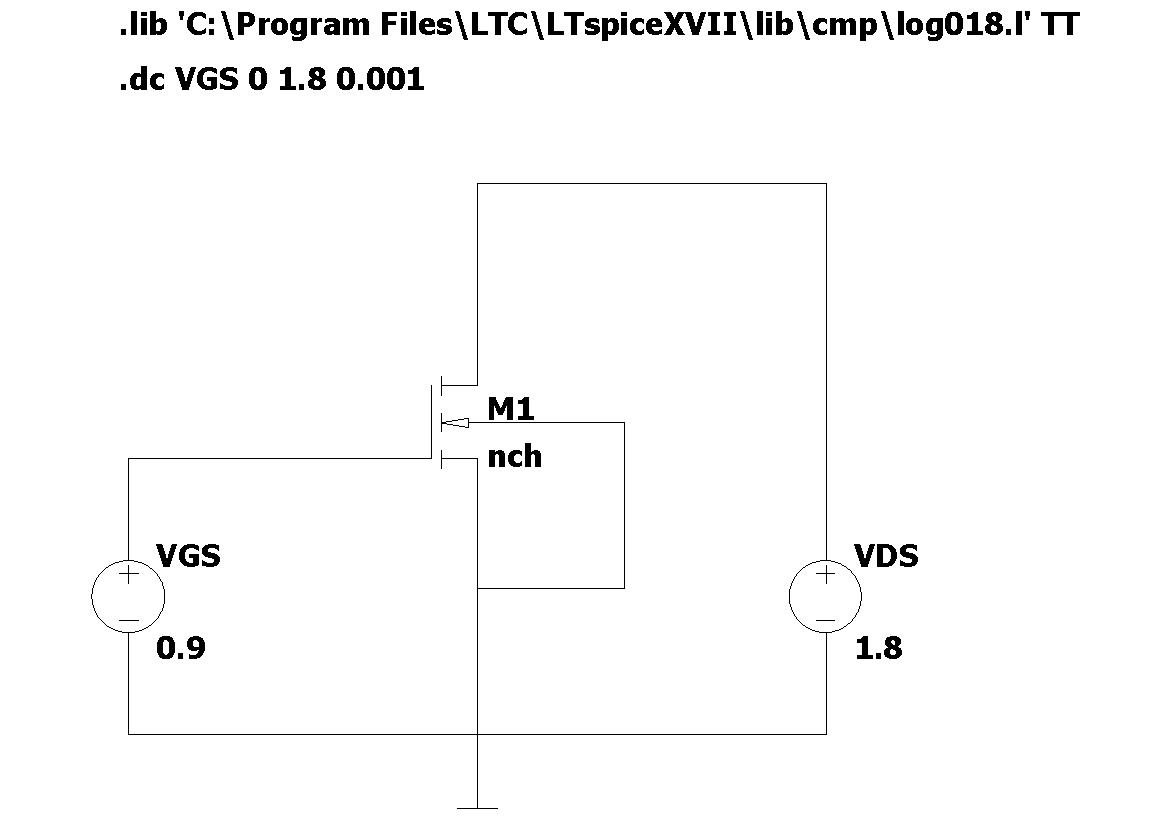
\includegraphics[width=300px]{img/q3/a/nmos-testbench.pdf}
\caption{\label{fig:nmos-testbench}NMOS Testbench}
\end{figure}
\item I\textsubscript{D}-V\textsubscript{GS}
\begin{figure}[H]
\centering
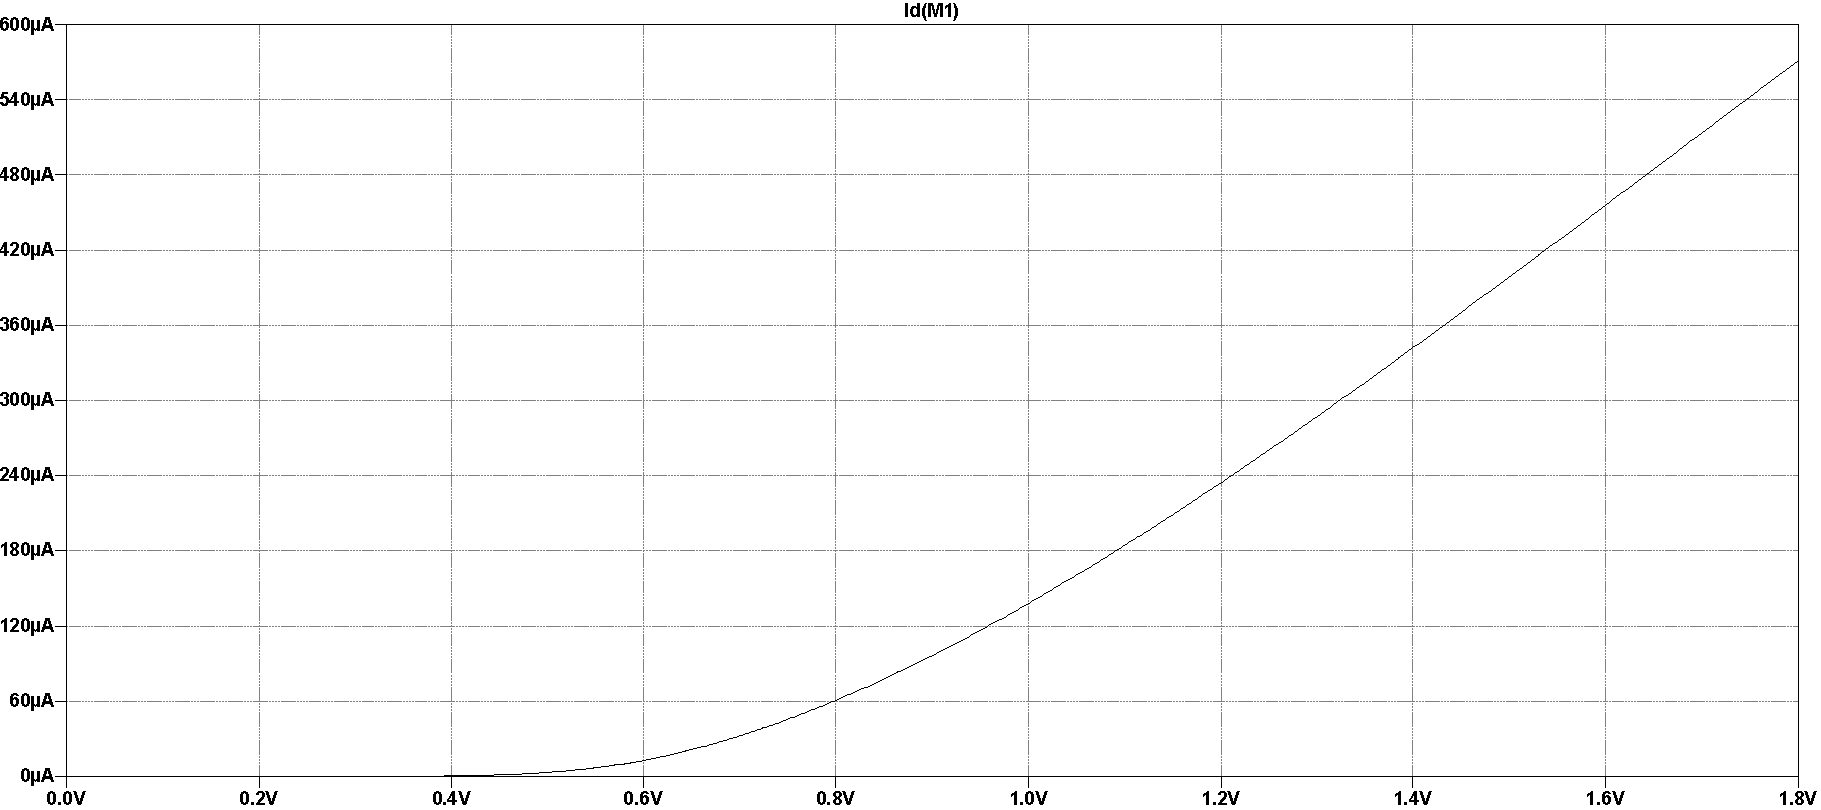
\includegraphics[width=.9\linewidth]{img/q3/a/nmos-id-vgs.pdf}
\caption{\label{fig:nmos-id-vgs}NMOS I\textsubscript{D}-V\textsubscript{GS}}
\end{figure}
\end{enumerate}
\item PMOS
\begin{enumerate}
\item Testbench
\begin{figure}[H]
\centering
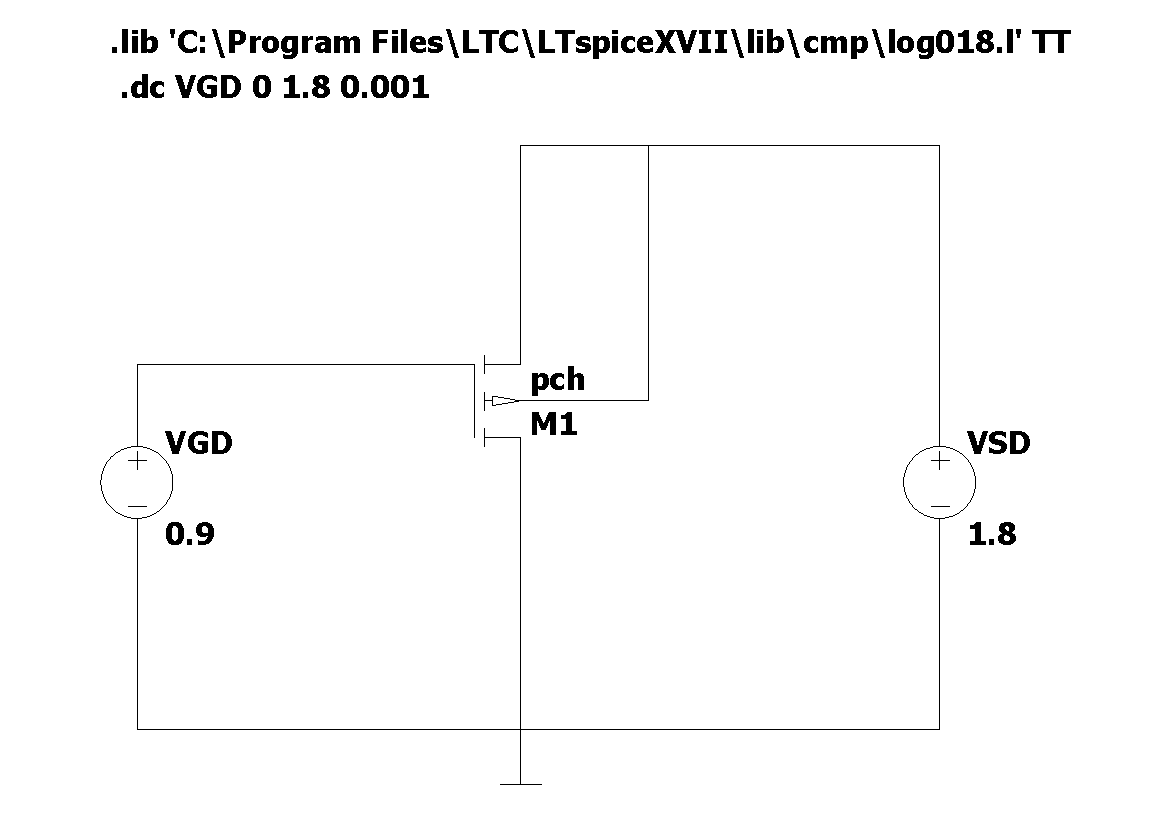
\includegraphics[width=300px]{img/q3/a/pmos-testbench.pdf}
\caption{\label{fig:pmos-testbench}PMOS Testbench}
\end{figure}
\item I\textsubscript{S}-V\textsubscript{GS}
\begin{figure}[H]
\centering
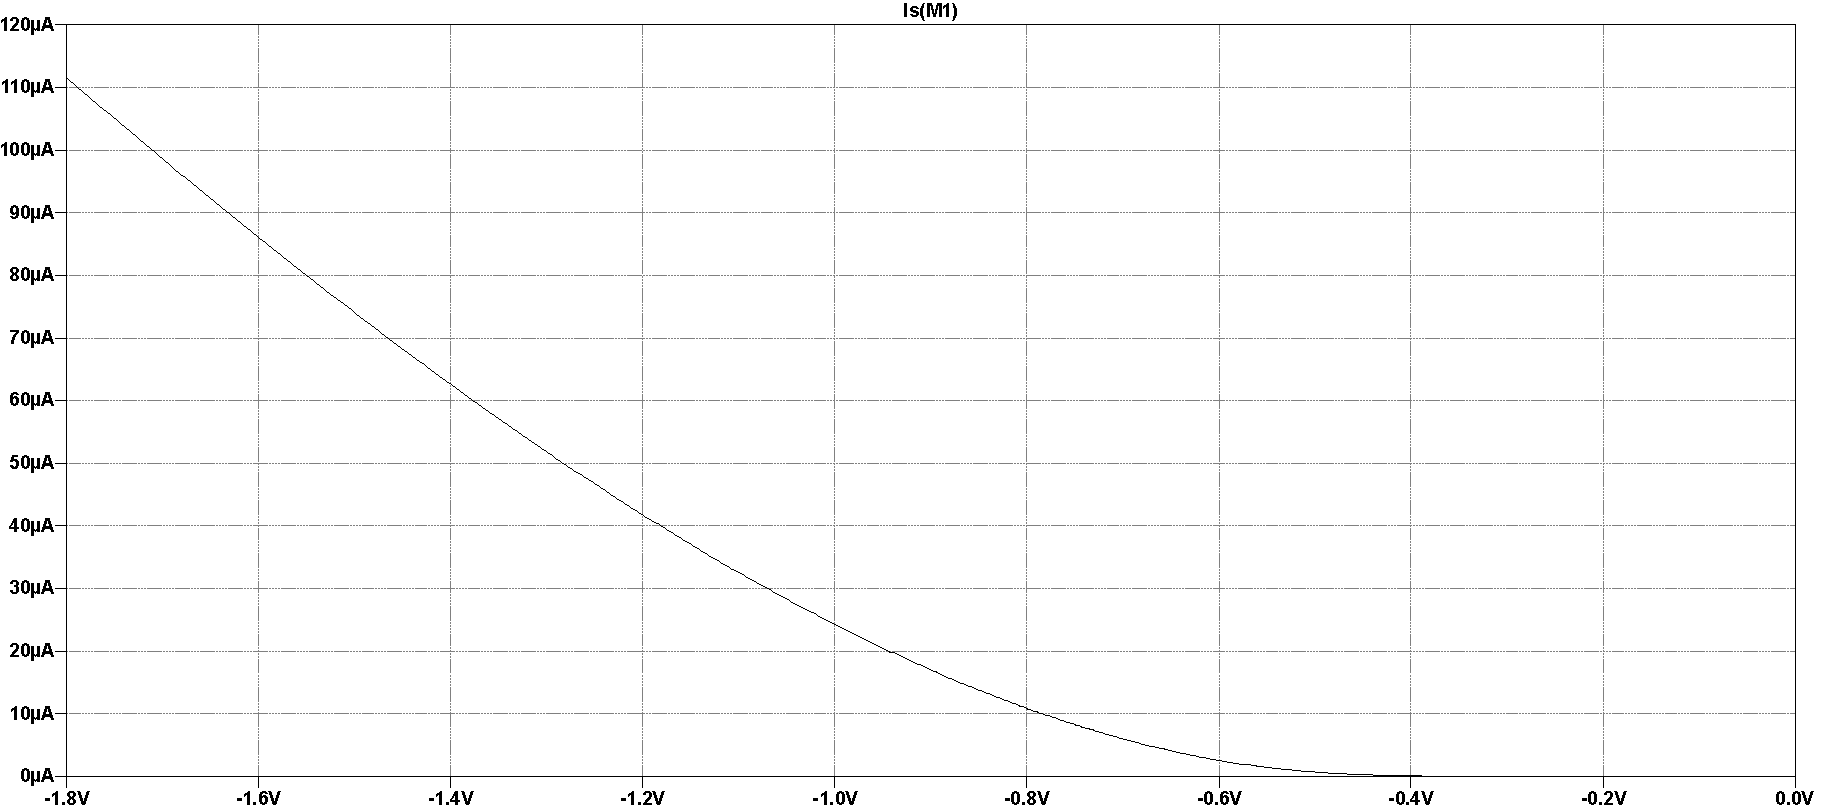
\includegraphics[width=.9\linewidth]{img/q3/a/pmos-is-vgs.pdf}
\caption{\label{fig:pmos-is-vgs}PMOS I\textsubscript{S}-V\textsubscript{GS}}
\end{figure}
\end{enumerate}
\end{enumerate}
\item \(\mu_{n(p)}C_{OX}\) and \(V_{THn(p)}\)

Assuming that channel length modulation is negligible, \(V_{THn}\) for NMOS can be derived
from the following relation:
\begin{equation*}
\begin{aligned}
I_{D} &= \frac{\mu_{n}C_{ox}}{2} \frac{W}{L} (V_{GS} - V_{THn})^2 \\
\frac{2 I_{D}}{\mu_{n}C_{ox}}\frac{L}{W} &=  (V_{GS} - V_{THn})^2 \\
\sqrt{\frac{2 I_{D}}{\mu_{n}C_{ox}}\frac{L}{W}} &=  V_{GS} - V_{THn} \\
\end{aligned}
\end{equation*}
V\textsubscript{THn} is the x-axis intercept when the saturation region is extrapolated.
In the case of PMOS, the relation becomes:
\begin{equation*}
\begin{aligned}
\sqrt{\frac{2 I_{S}}{\mu_{p}C_{ox}}\frac{L}{W}} &=  V_{SG} + V_{THp} \\
\end{aligned}
\end{equation*}
For deriving \(\mu_{n}C_{OX}\), since V\textsubscript{THn(p)} is constant at specific temperatures.
Differentiating both sides with respect to V\textsubscript{GS(SG)} will give:
\begin{equation*}
\begin{aligned}
\frac{d}{dV_{GS}}\sqrt{\frac{2 I_{D}}{\mu_{n}C_{ox}}\frac{L}{W}} &=  \frac{d}{dV_{GS}}(V_{GS} - V_{THn}) \\
\frac{1}{2} \frac{dI_{D}}{dV_{GS}} \sqrt{\frac{2}{I_{D}\mu_{n}C_{ox}}\frac{L}{W}} &=  1 \\
\sqrt{\mu_{n}C_{ox}} &= \frac{1}{2} \frac{dI_{D}}{dV_{GS}} \sqrt{\frac{2}{I_{D}}\frac{L}{W}} \\
\mu_{n}C_{ox} &= \frac{1}{2} \frac{L}{W} \frac{1}{I_{D}}(\frac{dI_{D}}{dV_{GS}})^{2} \\
\mu_{n}C_{ox} &= \frac{1}{6 I_{D}}(\frac{dI_{D}}{dV_{GS}})^{2} \\
\end{aligned}
\end{equation*}
In the case for PMOS, the relation becomes:
\begin{equation*}
\begin{aligned}
\mu_{p}C_{ox} &= \frac{1}{6 I_{S}}(\frac{dI_{S}}{dV_{SG}})^{2} \\
\end{aligned}
\end{equation*}

\begin{enumerate}
\item NMOS
\begin{enumerate}
\item \(\mu_{n}C_{OX}\)

\begin{figure}[H]
\centering
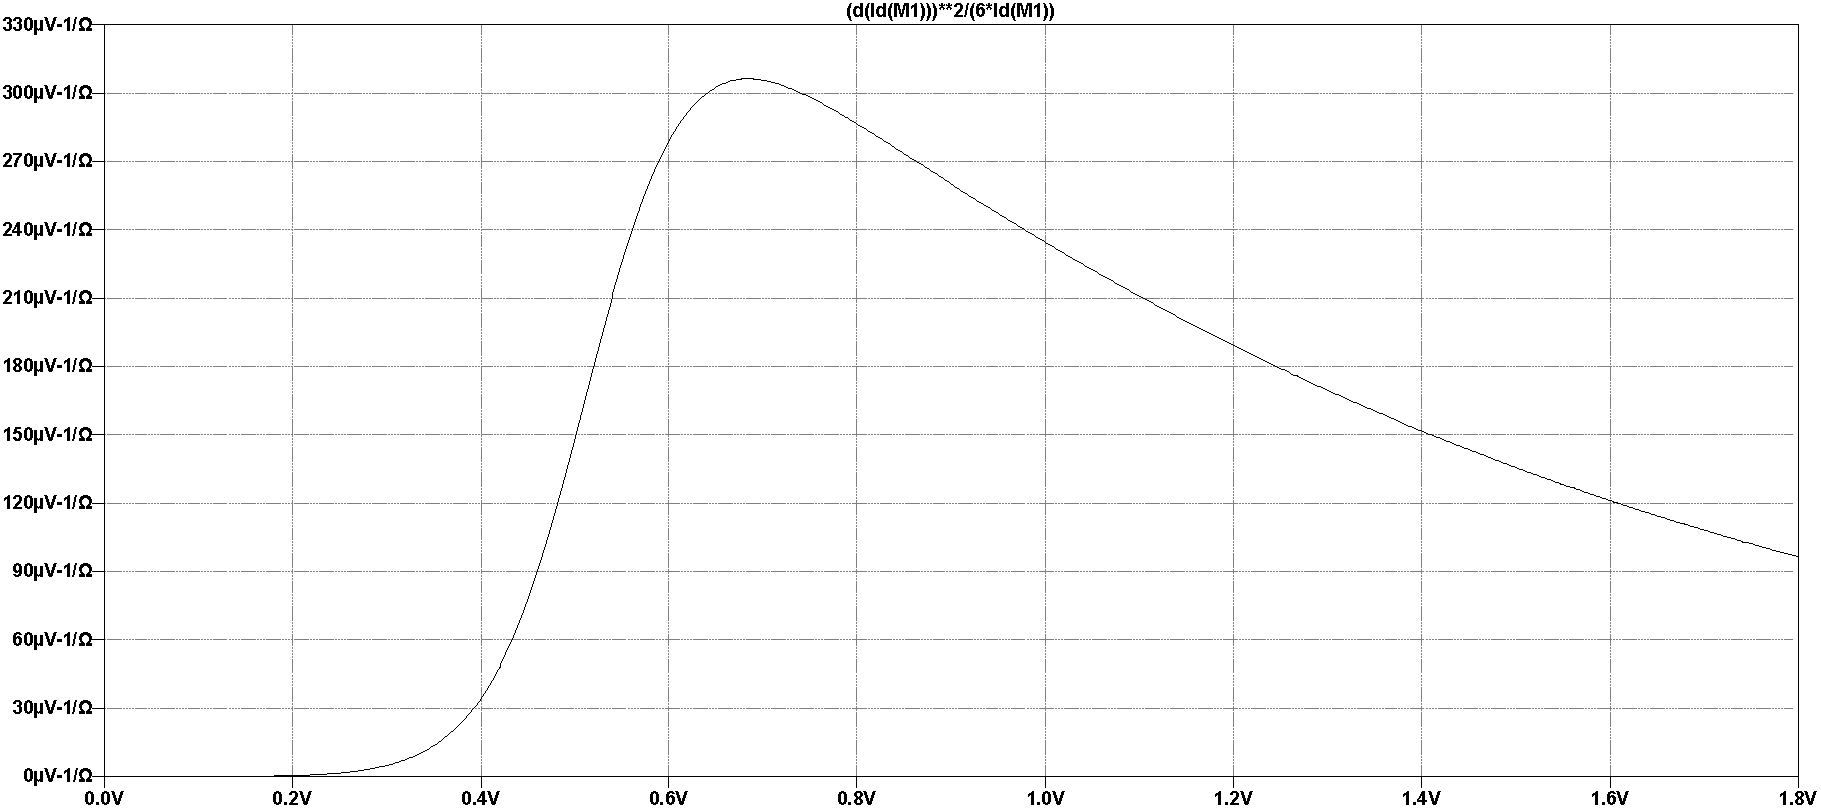
\includegraphics[width=.9\linewidth]{img/q3/b/nmos-ucox-vgs.pdf}
\caption{\label{fig:nmos-ucox-vgs}NMOS \(\mu\)\textsubscript{n}C\textsubscript{OX}-V\textsubscript{GS}}
\end{figure}
\item \(V_{THn} = 0.44V\)
\begin{figure}[H]
\centering
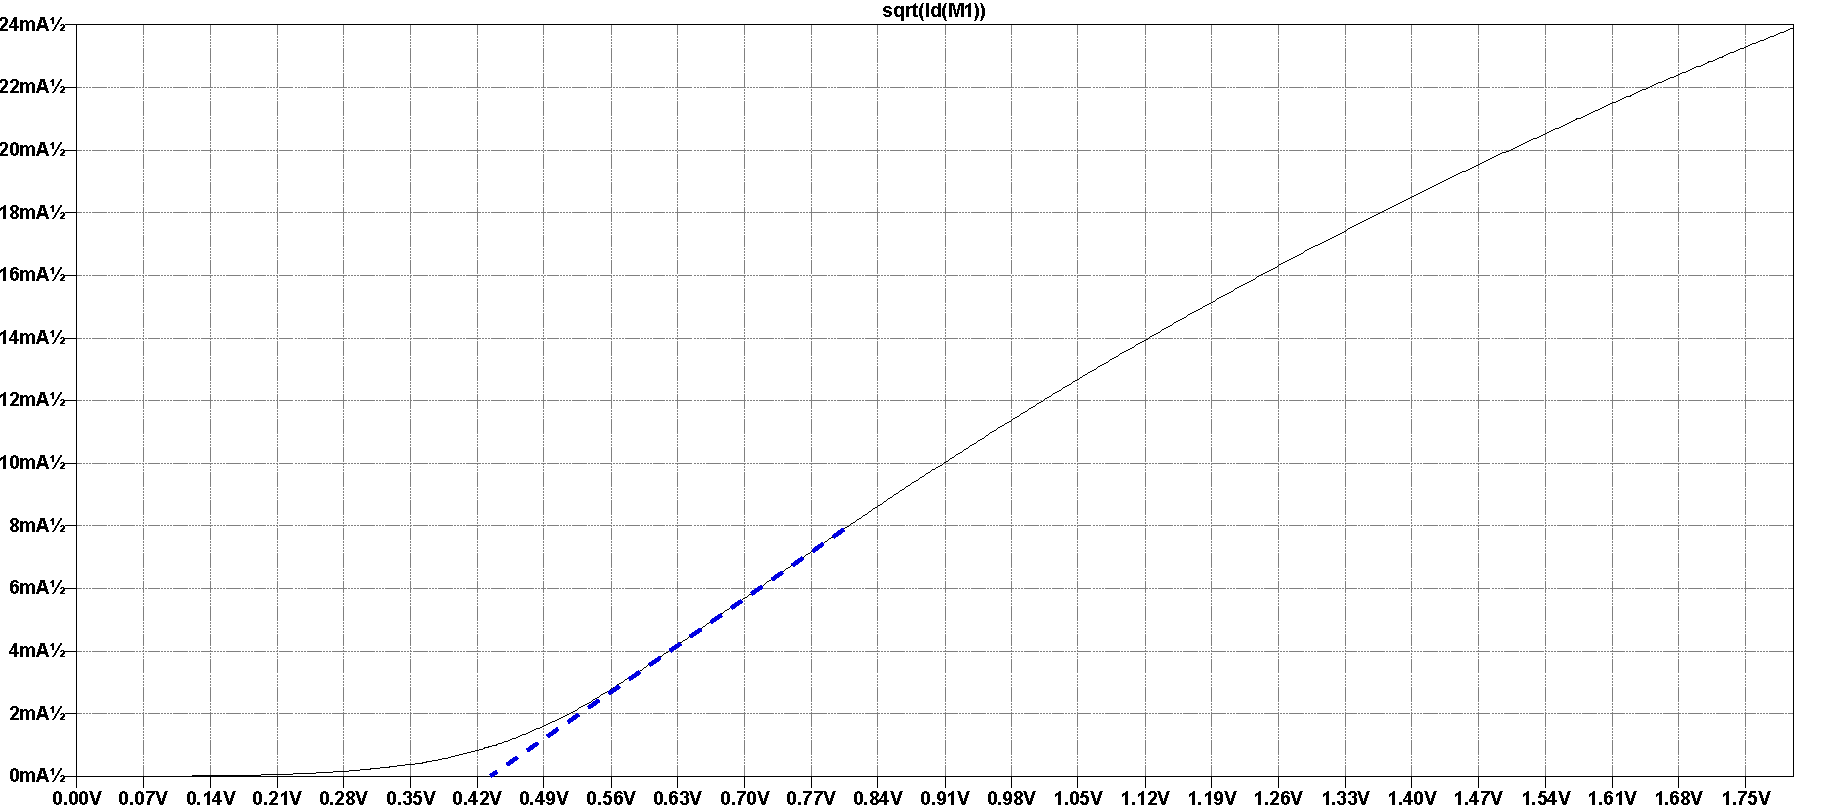
\includegraphics[width=.9\linewidth]{img/q3/b/nmos-sqrt-id-vgs.pdf}
\caption{\label{fig:nmos-sqrt-id-vgs}NMOS \(\sqrt{I_{D}}-V_{GS}\)}
\end{figure}
\end{enumerate}
\item PMOS
\begin{enumerate}
\item \(\mu_{p}C_{OX}\)

\begin{figure}[H]
\centering
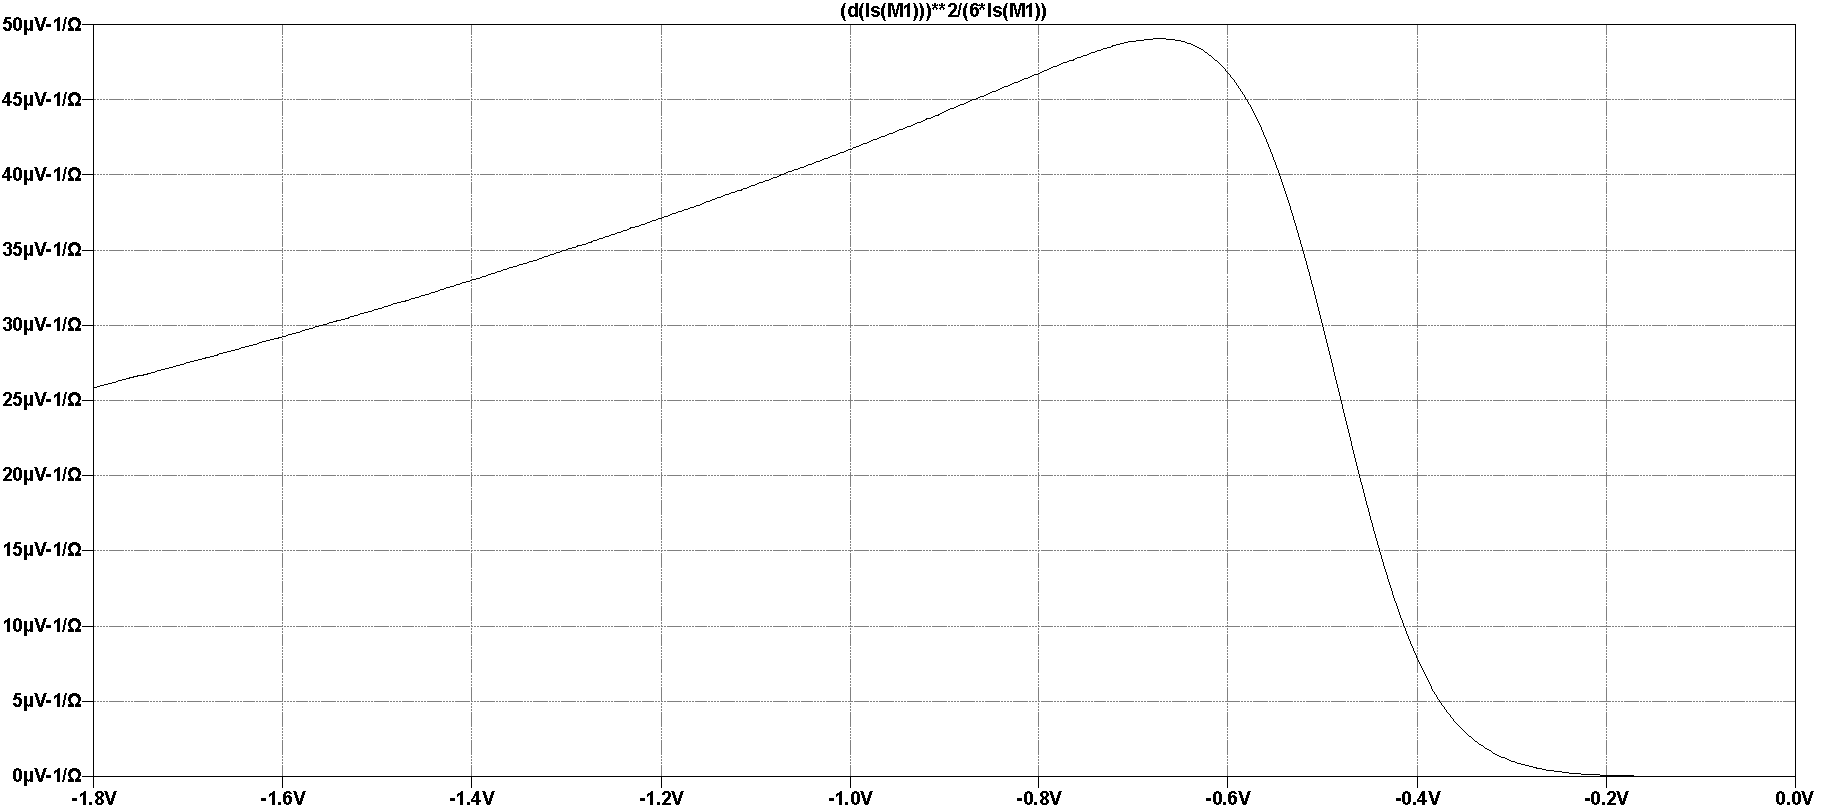
\includegraphics[width=.9\linewidth]{img/q3/b/pmos-ucox-vgs.pdf}
\caption{\label{fig:pmos-ucox-vgs}PMOS \(\mu\)\textsubscript{p}C\textsubscript{OX}-V\textsubscript{GS}}
\end{figure}
\item \(V_{THp} = -0.42V\)
\begin{figure}[H]
\centering
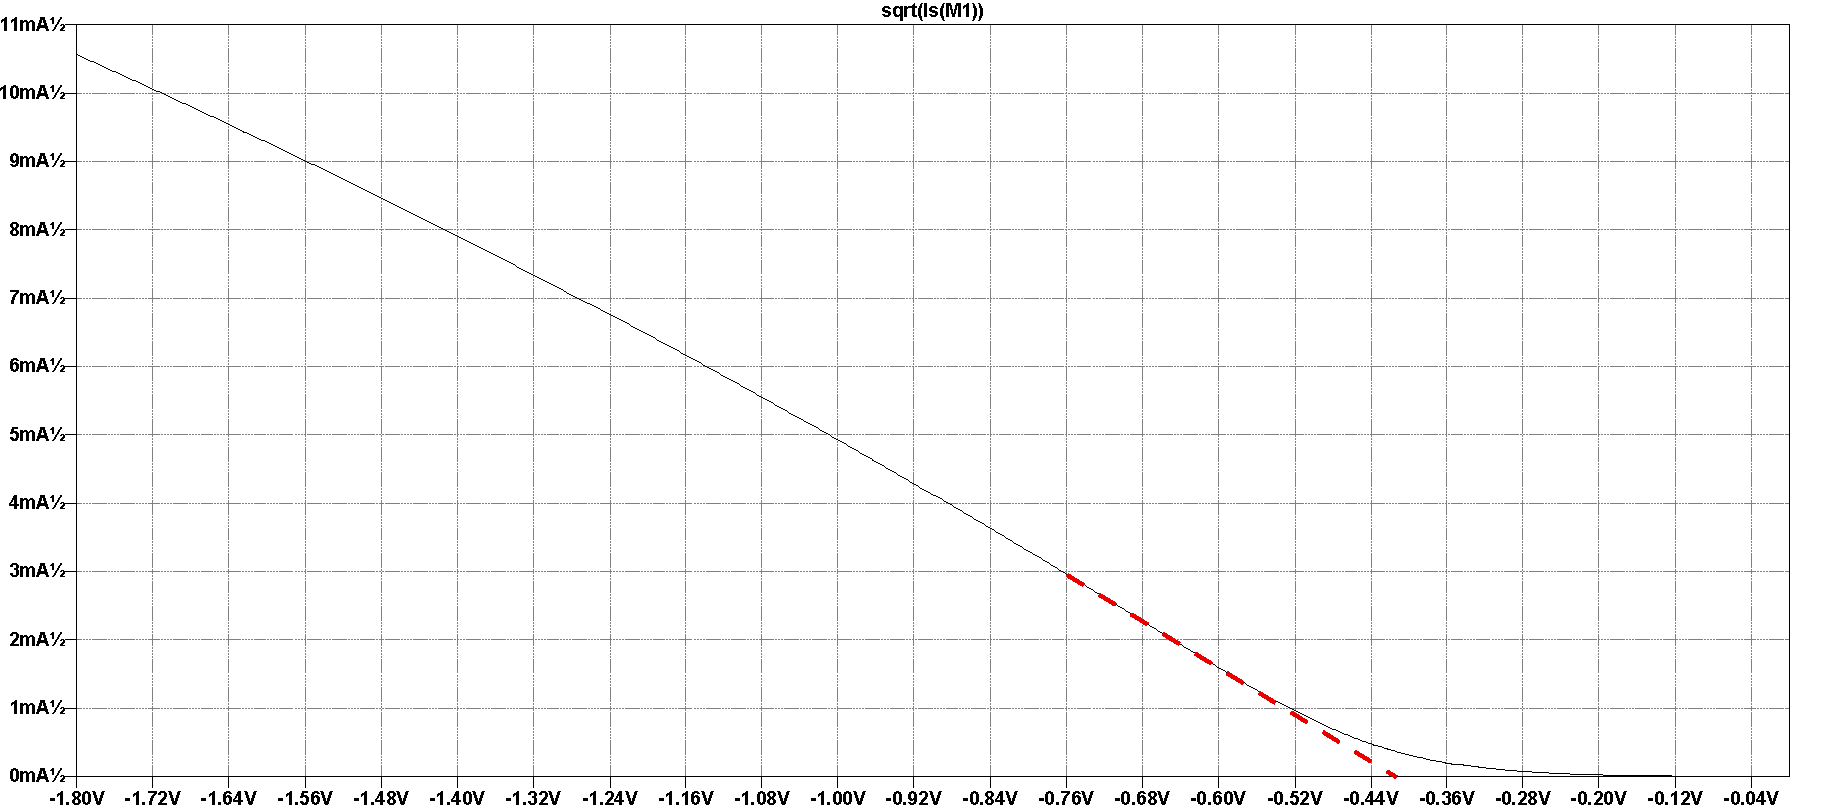
\includegraphics[width=.9\linewidth]{img/q3/b/pmos-sqrt-is-vgs.pdf}
\caption{\label{fig:nmos-sqrt-is-vgs}PMOS \(\sqrt{I_{S}}-V_{GS}\)}
\end{figure}
\end{enumerate}
\end{enumerate}
\end{enumerate}

\section{Problem 4}
\label{sec:org2ebaa55}
\begin{enumerate}
\item Testbench and I\textsubscript{D}-V\textsubscript{DS} characteristics of NMOS and PMOS
\begin{enumerate}
\item NMOS
\begin{enumerate}
\item Testbench
\begin{figure}[H]
\centering
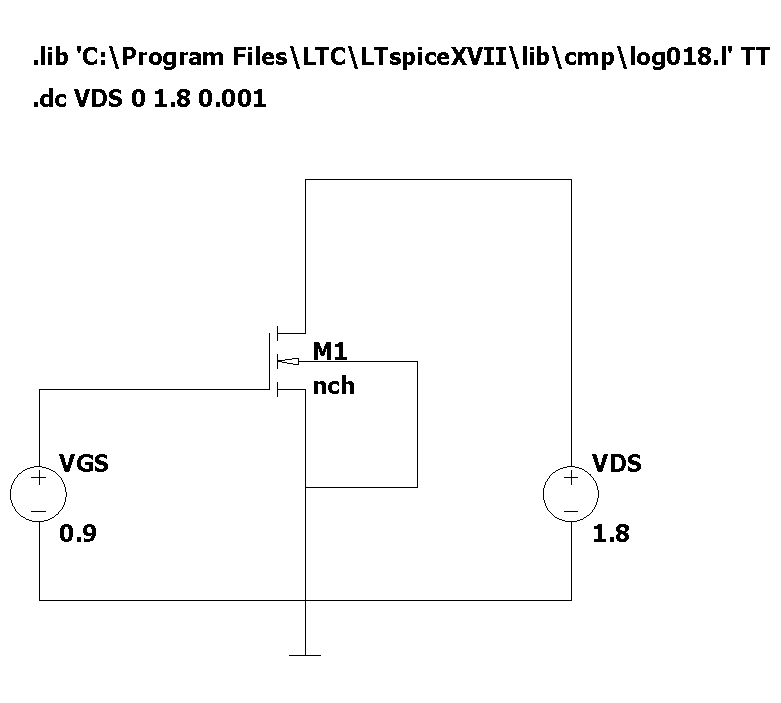
\includegraphics[width=300px]{img/q4/a/nmos-testbench.pdf}
\caption{\label{fig:nmos-testbench-2}NMOS Testbench}
\end{figure}
\item I\textsubscript{D}-V\textsubscript{DS} characteristics
\begin{figure}[H]
\centering
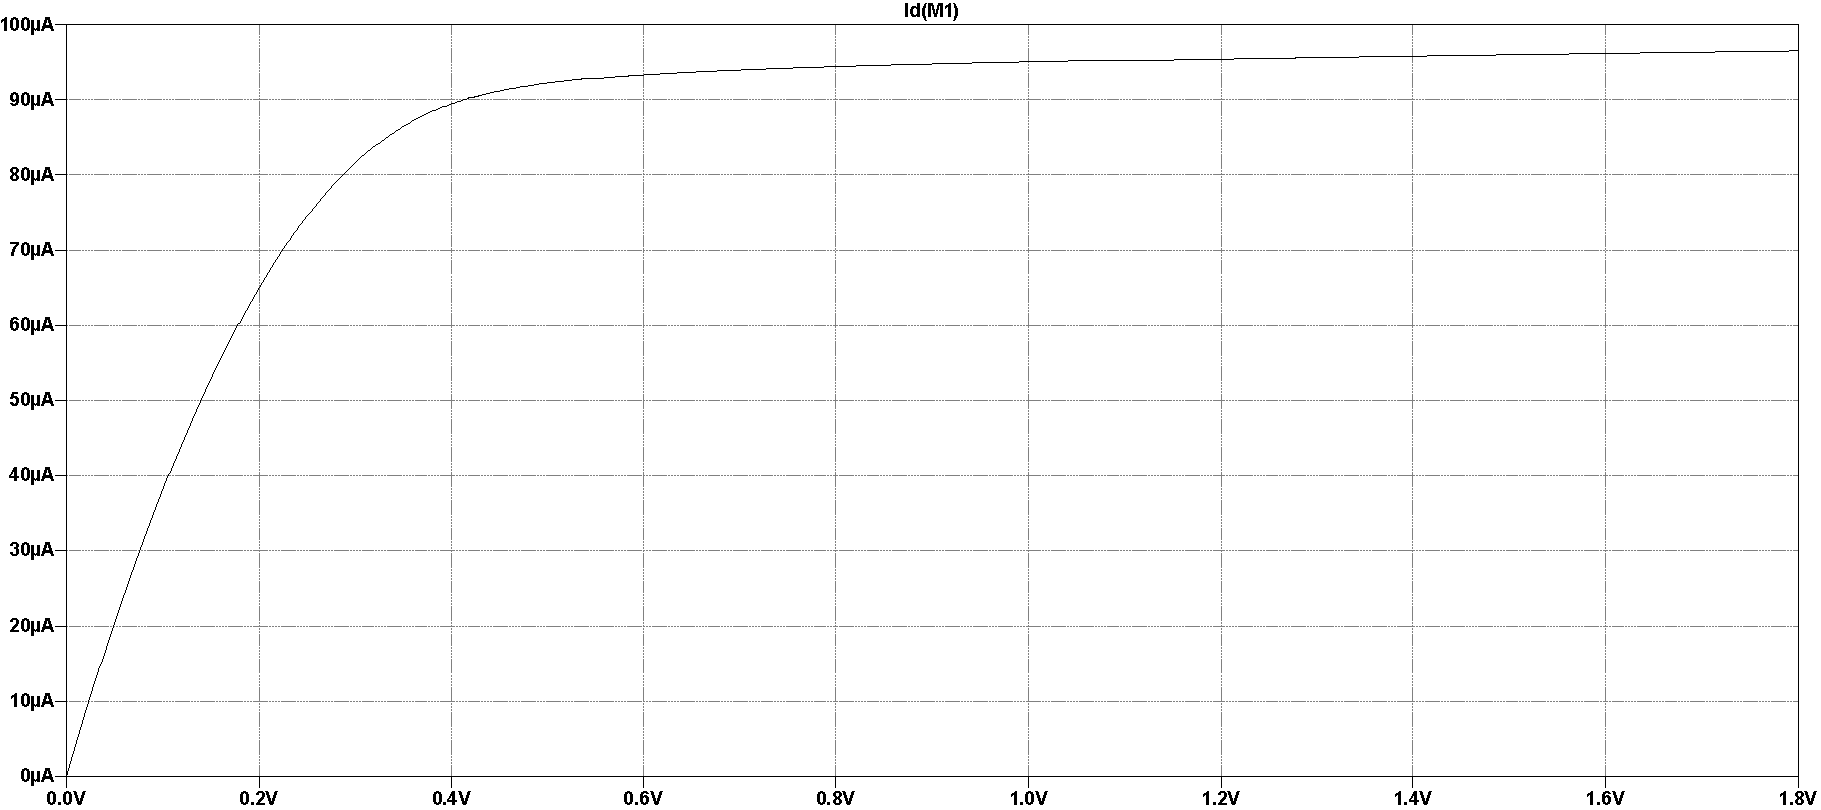
\includegraphics[width=.9\linewidth]{img/q4/a/nmos-id-vds.pdf}
\caption{\label{fig:nmos-id-vds}NMOS I\textsubscript{D}-V\textsubscript{DS}}
\end{figure}
\end{enumerate}
\item PMOS
\begin{enumerate}
\item Testbench
\begin{figure}[H]
\centering
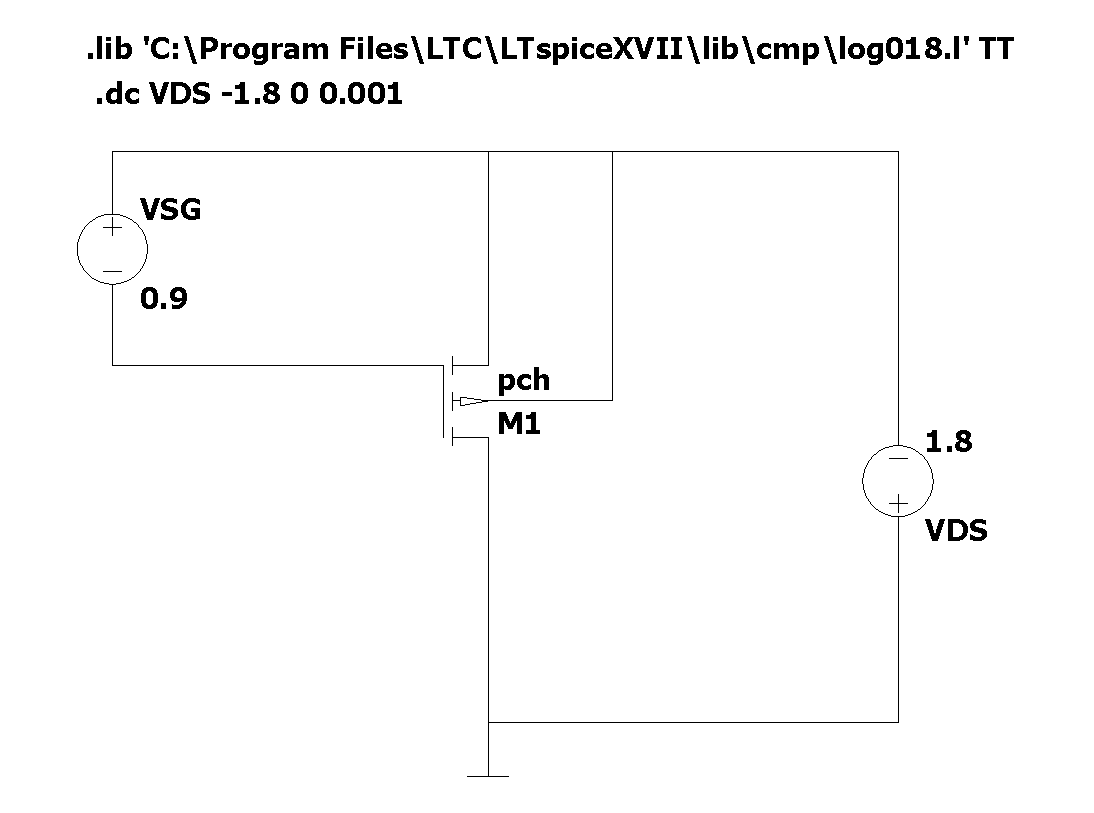
\includegraphics[width=300px]{img/q4/a/pmos-testbench.pdf}
\caption{\label{fig:pmos-testbench-2}PMOS Testbench}
\end{figure}
\item I\textsubscript{S}-V\textsubscript{DS} characteristics
\begin{figure}[H]
\centering
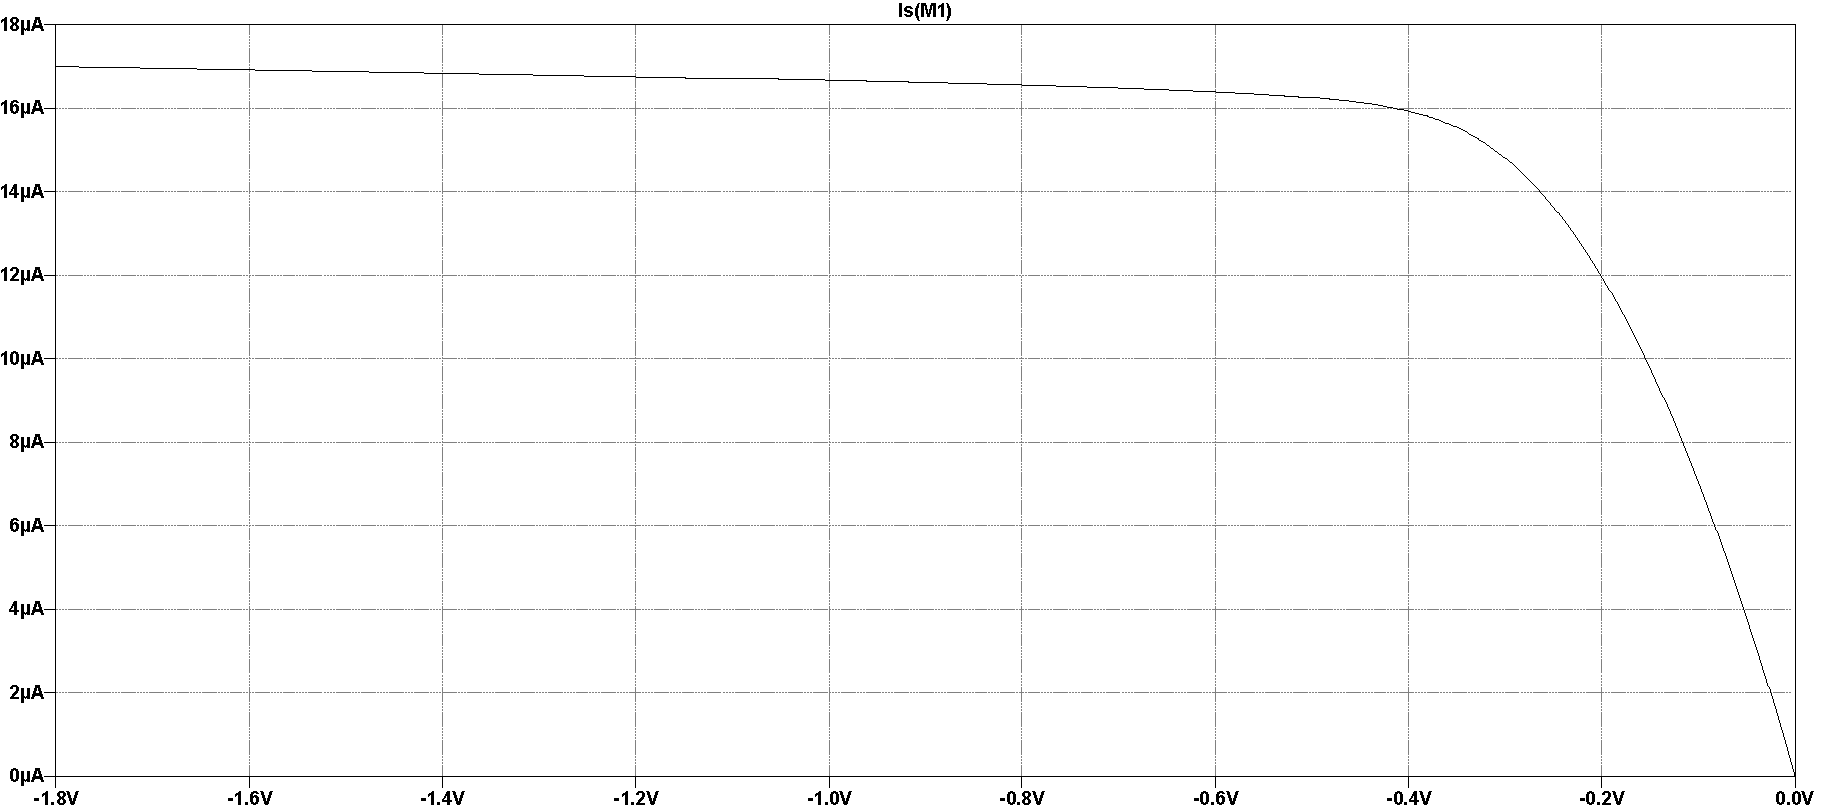
\includegraphics[width=.9\linewidth]{img/q4/a/pmos-is-vds.pdf}
\caption{\label{fig:nmos-id-vds}PMOS I\textsubscript{S}-V\textsubscript{DS}}
\end{figure}
\end{enumerate}
\end{enumerate}
\item \(\lambda_{n(p)}\)

Drain current characteristics for NMOS under saturation conditions:
\begin{equation*}
\begin{aligned}
I_{D} &= \frac{\mu_{n}C_{ox}}{2} \frac{W}{L} (V_{GS} - V_{TH})^2(1 + \lambda_{n}V_{DS}) \\
\end{aligned}
\end{equation*}
Differentiating both side with respect to V\textsubscript{DS}.
\begin{equation*}
\begin{aligned}
\frac{dI_{D}}{dV_{DS}} &= \frac{d}{dV_{DS}} (\frac{\mu_{n}C_{ox}}{2} \frac{W}{L} (V_{GS} - V_{TH})^2(1 + \lambda_{n} V_{DS})) \\
\frac{dI_{D}}{dV_{DS}} &= \frac{\mu_{n}C_{ox}}{2} \frac{W}{L} (V_{GS} - V_{TH})^2 \lambda_{n} \\
\end{aligned}
\end{equation*}
Assuming that the body-effect is small:
\begin{equation*}
\begin{aligned}
I_{D} &\approx \frac{\mu_{n}C_{ox}}{2} \frac{W}{L} (V_{GS} - V_{TH})^2 \\
\\
\frac{dI_{D}}{dV_{DS}} &\approx I_{D} \lambda_{n} \\
\lambda_{n} &\approx \frac{1}{I_{D}} \frac{dI_{D}}{dV_{DS}}
\end{aligned}
\end{equation*}
In the case of PMOS:
\begin{equation*}
\begin{aligned}
\lambda_{p} &\approx \frac{1}{I_{S}} \frac{dI_{S}}{dV_{SD}}
\end{aligned}
\end{equation*}

\begin{enumerate}
\item \(\lambda_{n} = 0.18 V^{-1}\)
\begin{figure}[H]
\centering
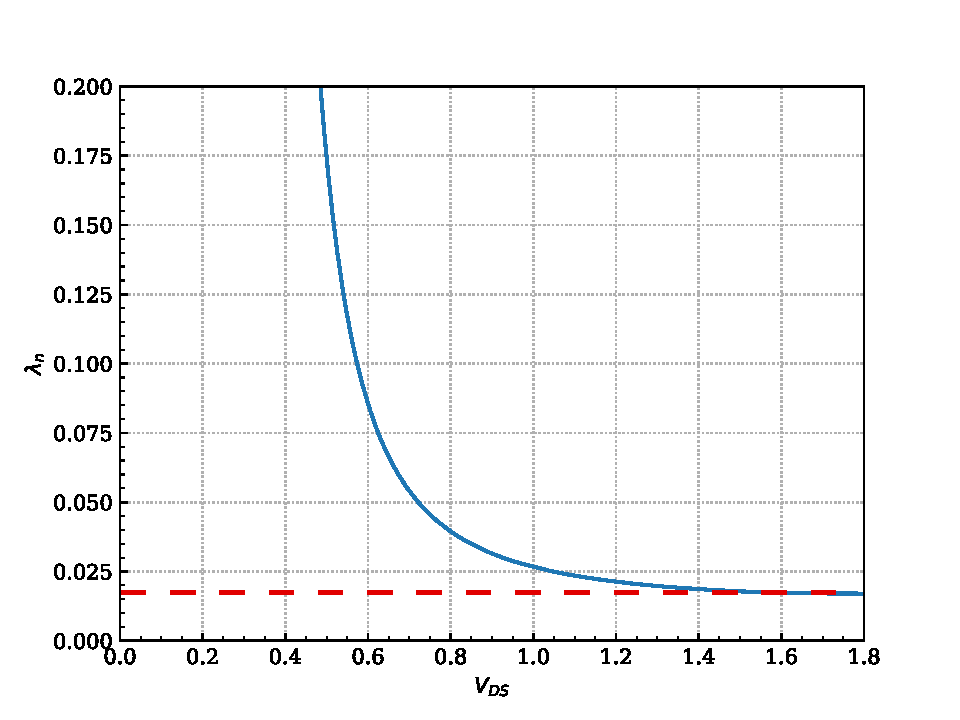
\includegraphics[width=350px]{img/q4/b/nmos-d-id-id.pdf}
\caption{\label{fig:nmos-d-id-id}NMOS \(\lambda_{n}-V_{DS}\)}
\end{figure}

\item \(\lambda_{p} = - 0.022 V^{-1}\)
\begin{figure}[H]
\centering
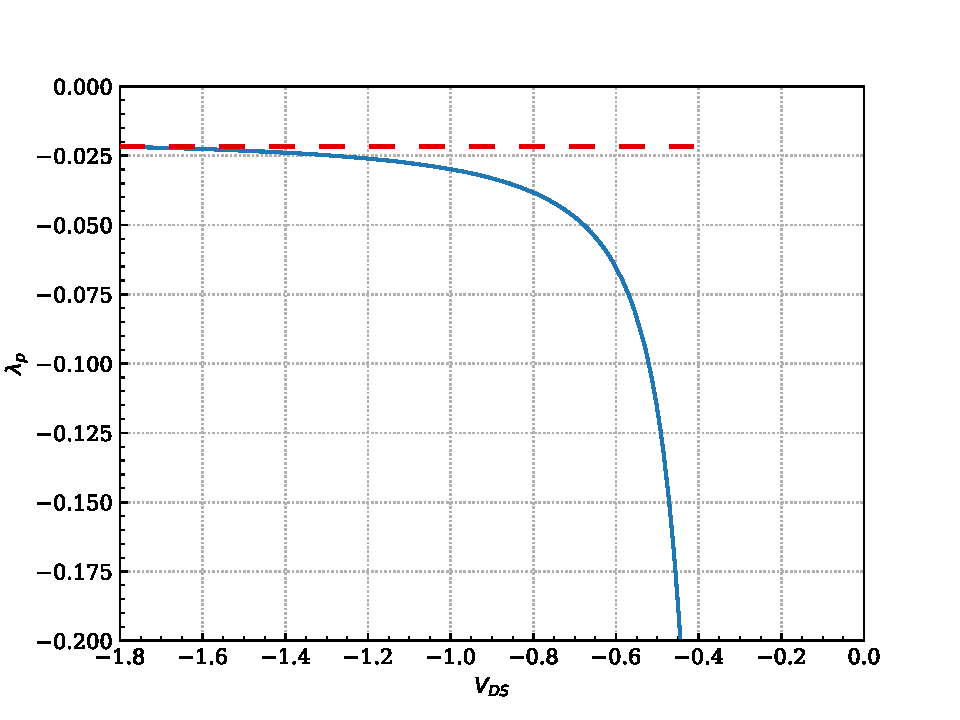
\includegraphics[width=350px]{img/q4/b/pmos-d-is-is.pdf}
\caption{\label{fig:nmos-d-is-is}PMOS \(\lambda_{p}-V_{DS}\)}
\end{figure}
\end{enumerate}
\end{enumerate}
\section{Problem 5}
\label{sec:org13acd5e}
g\textsubscript{m} for NMOS is approximately:
\begin{equation*}
\begin{align}
g_{m} &\approx \frac{\partial{I_{D}}}{\partial{V_{GS}}}
\end{align}
\end{equation*}
For PMOS:
\begin{equation*}
\begin{align}
g_{m} &\approx \frac{\partial{I_{S}}}{\partial{V_{SG}}}
\end{align}
\end{equation*}
\begin{enumerate}
\item \(\frac{g_{m}}{I_{D}}-V_{GS}\)
\begin{enumerate}
\item NMOS
\begin{figure}[H]
\centering
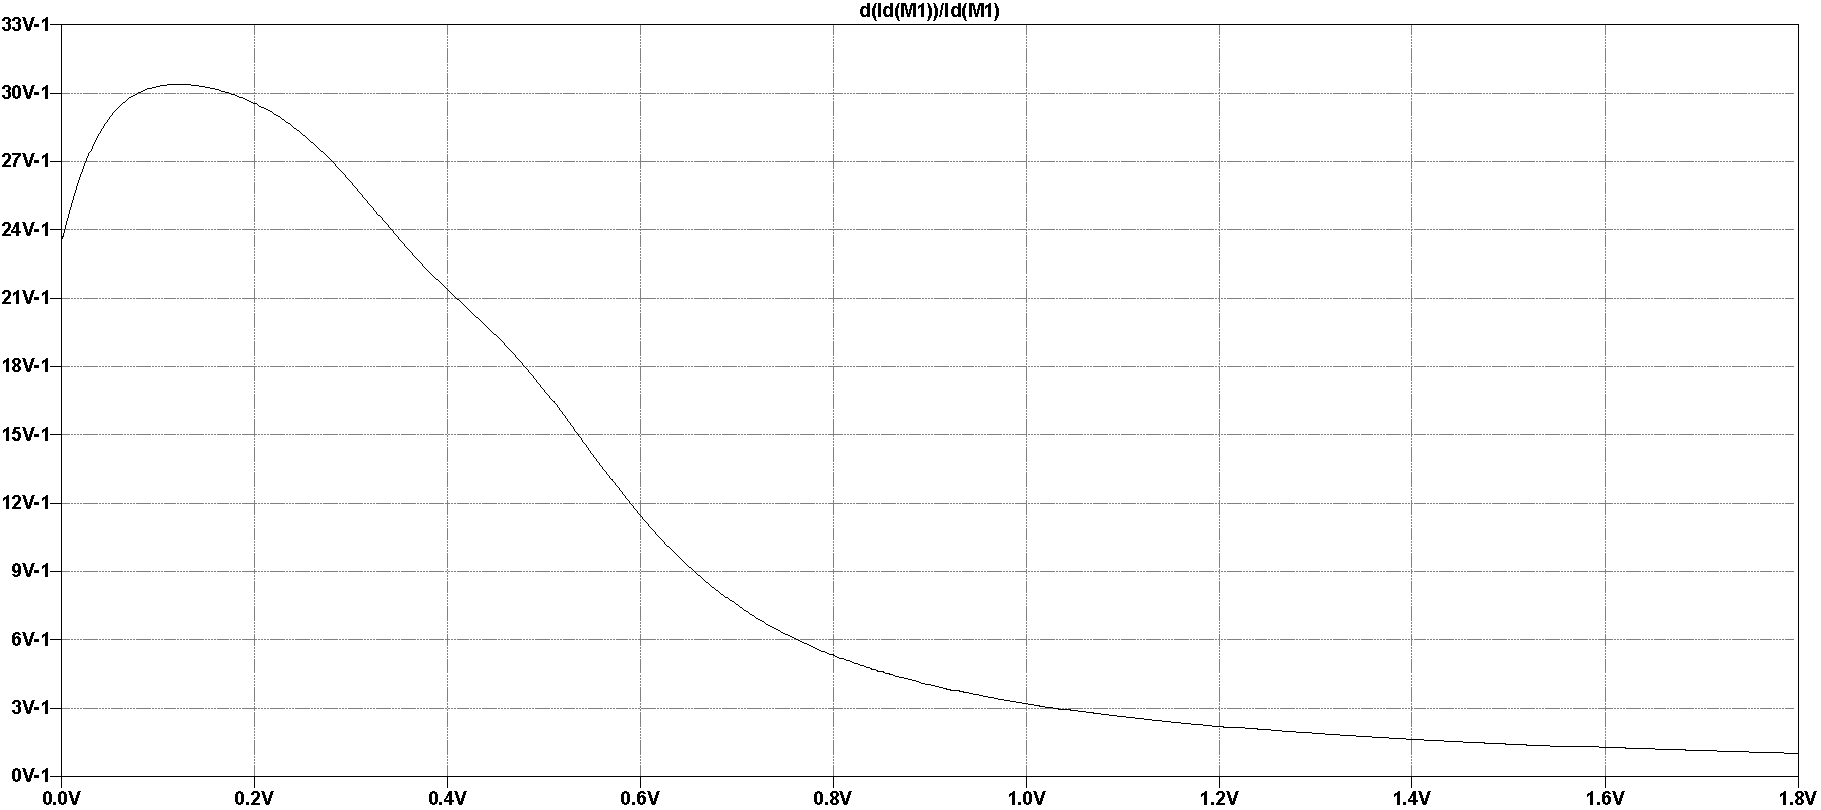
\includegraphics[width=.9\linewidth]{img/q5/a/nmos-d-id-id-vgs.pdf}
\caption{\label{fig:nmos-d-id-id-vgs}NMOS \(\frac{g_{m}}{I_{D}}-V_{GS}\)}
\end{figure}
\item PMOS
\begin{figure}[H]
\centering
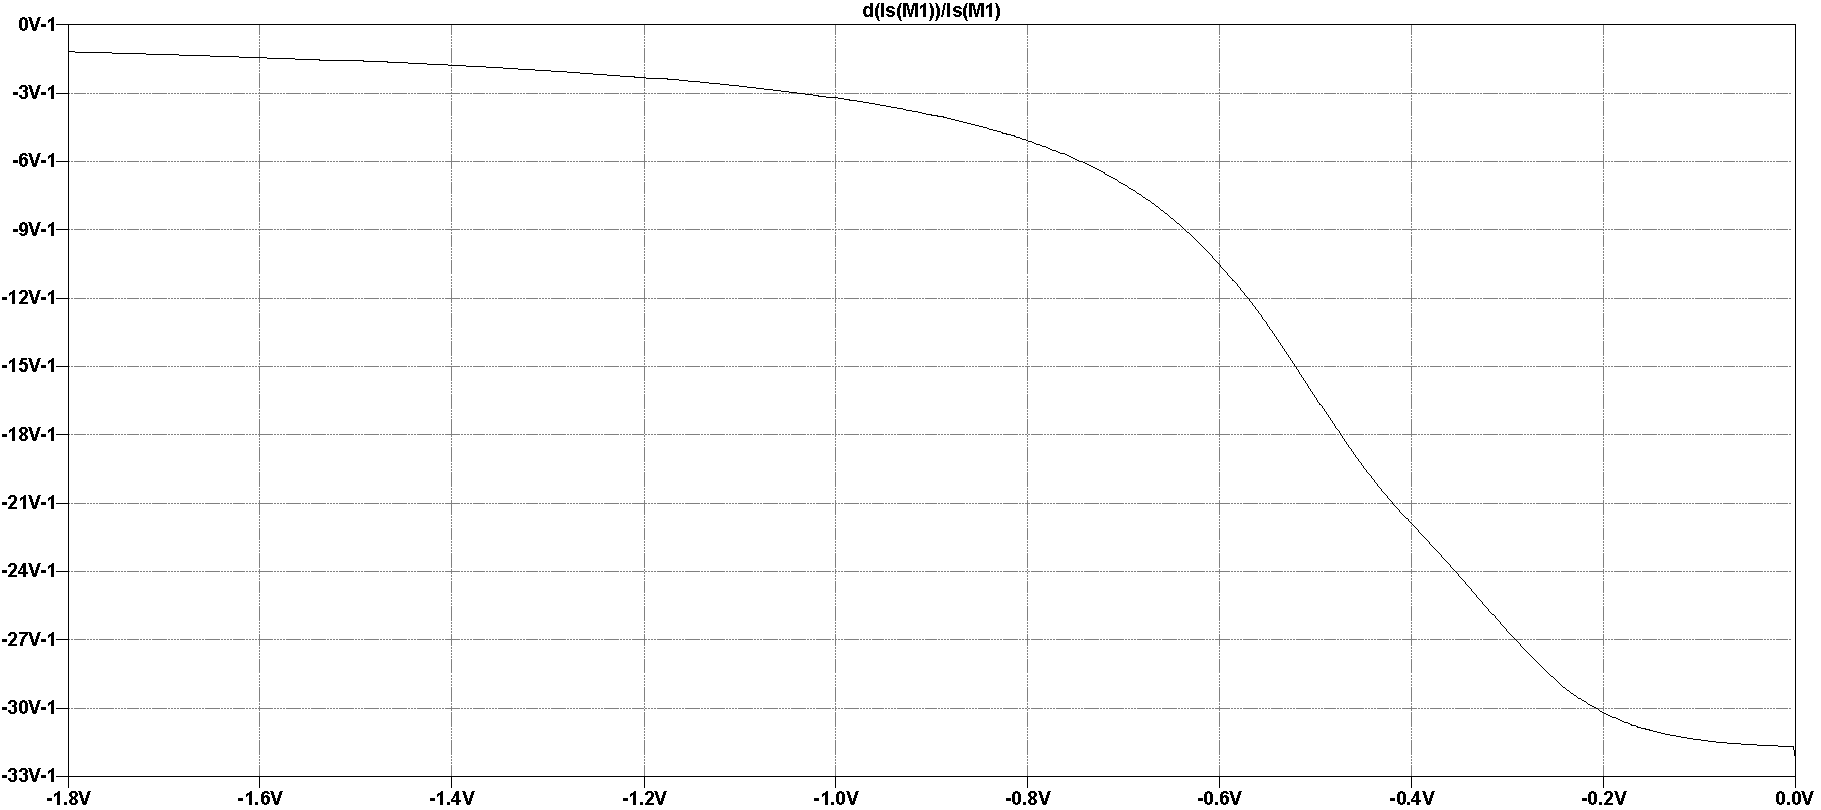
\includegraphics[width=.9\linewidth]{img/q5/a/pmos-d-is-is-vgs.pdf}
\caption{\label{fig:pmos-d-is-is-vgs}PMOS \(\frac{g_{m}}{I_{S}}-V_{GS}\)}
\end{figure}
\end{enumerate}
\item \(max(|\frac{g_{m}}{I_{D(S)}}|)\)
\begin{enumerate}
\item NMOS

\(max(|\frac{g_{m}}{I_{D}}|) = 30.4 V^{-1}\)
\item PMOS

\(max(|\frac{g_{m}}{I_{S}}|) = 31.7 V^{-1}\)
\end{enumerate}
\item Slope factor, n
\begin{enumerate}
\item NMOS
\begin{equation*}
\begin{aligned}
max(|\frac{g_{m}}{I_{D}}|) &= 30.4 V^{-1}\\\\
\frac{1}{nV_{t}} &= 30.4 V^{-1}\\
n &= \frac{1}{0.026 \times 30.4}\\
n &= 1.27 \\
\end{aligned}
\end{equation*}
\item PMOS
\begin{equation*}
\begin{aligned}
max(|\frac{g_{m}}{I_{S}}|) &= 31.7 V^{-1}\\\\
\frac{1}{nV_{t}} &= 31.7 V^{-1}\\
n &= \frac{1}{0.026 \times 31.7}\\
n &= 1.21 \\
\end{aligned}
\end{equation*}
\end{enumerate}
\end{enumerate}

\section{Problem 6}
\label{sec:orgf432feb}
\begin{enumerate}
\item Small-signal Model
\begin{figure}[H]
\centering
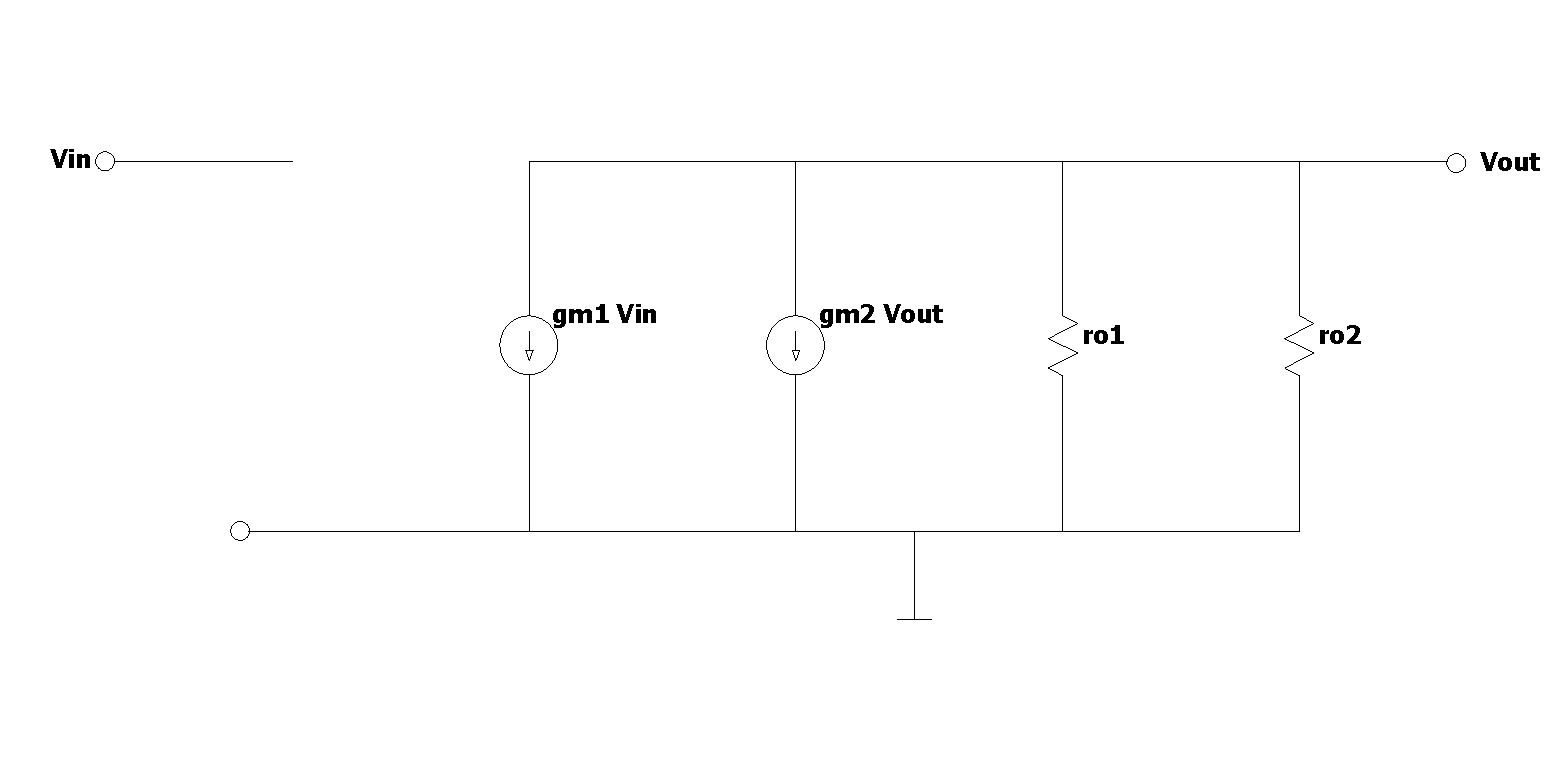
\includegraphics[width=350px]{img/q6/a/small-signal-model.pdf}
\caption{\label{fig:small-signal-model}Small signal model}
\end{figure}
\item \(\lambda = 0 V^{-1}\)
\begin{enumerate}
\item \(A_{V} = \frac{v_{out}}{v_{in}}\)
\begin{equation*}
\begin{aligned}
(g_{m1}v_{in} + g_{m2} v_{out}) &= 0 \\
A_{V} = \frac{v_{out}}{v_{in}} &= -\frac{g_{m1}}{g_{m2}} \\
\end{aligned}
\end{equation*}
\item \(R_{out}\)
\begin{equation*}
\begin{aligned}
R_{out} &= \frac{1}{g_{m2}}
\end{aligned}
\end{equation*}
\end{enumerate}
\item \(\lambda \neq 0 V^{-1}\)
\begin{enumerate}
\item \(A_{V} = \frac{v_{out}}{v_{in}}\)
\begin{equation*}
\begin{aligned}
-v_{out} &= (g_{m1}v_{in} + g_{m2} v_{out})(r_{o1} // r_{o2}) \\
-v_{in} g_{m1}(r_{o1} // r_{o2}) &= (1 + g_{m2} (r_{o1} // r_{o2}))v_{out} \\
A_{V} = \frac{v_{out}}{v_{in}} &= -\frac{g_{m1}}{g_{m2} + \frac{1}{r_{o1}} + \frac{1}{r_{o2}}}
\end{aligned}
\end{equation*}

\item \(R_{out}\)
\begin{equation*}
\begin{aligned}
R_{out} &= \frac{1}{g_{m2} + \frac{1}{r_{o1}} + \frac{1}{r_{o2}}}
\end{aligned}
\end{equation*}
\end{enumerate}
\end{enumerate}
\section{Problem 7}
\label{sec:org984d18d}
\begin{enumerate}
\item V\textsubscript{out}-V\textsubscript{in} relation when:
\begin{enumerate}
\item M\textsubscript{1} and M\textsubscript{2} under subthreshold conditions
\begin{equation*}
\begin{aligned}
V_{TH_{n}} &= 0.44 V \\
V_{TH_{p}} &= -0.42 V \\
\\
\mu_{n}C_{OX_{n}} &= 306 \mu{}AV^{-2} \\
\mu_{p}C_{OX_{p}} &= 49 \mu{}AV^{-2} \\
\\
n_{n} &= 1.27 \\
n_{p} &= 1.21 \\
\\
I_{D_{1}} &= I_{D_{2}} \\
(\mu_{n}C_{OX_{n}}(n - 1)\frac{W_{n}}{L_{n}}V_{T}^{2}) e^{\frac{V_{in} - V_{TH_{n}}}{n_{n}V_{T}}} &=
(\mu_{p}C_{OX_{p}}(n - 1)\frac{W_{p}}{L_{p}}V_{T}^{2}) e^{\frac{V_{DD} - V_{out} + V_{TH_{p}}}{n_{p}V_{T}}} \\
247 e^{\frac{V_{in} - 0.44}{0.033}} &= 154 e^{\frac{1.8 - V_{out} - 0.42}{0.031}} \\
ln(1.6) + \frac{V_{in} - 0.44}{0.033} &= \frac{1.38 - V_{out}}{0.031} \\
0.015 + V_{in} - 0.44 &\approx 1.38 - V_{out} \\
V_{out} &\approx 1.8V - V_{in} \\
\\
V_{in} &< 0.44 V
\end{aligned}
\end{equation*}

\item M\textsubscript{1} and M\textsubscript{2} at saturation
\begin{equation*}
\begin{aligned}
I_{D_{1}} &= I_{D_{2}} \\
\frac{\mu_{n}C_{OX_{n}}}{2}\frac{W_{n}}{L_{n}}(V_{GS_{1}} - V_{TH_{n}})^{2} &=
\frac{\mu_{p}C_{OX_{p}}}{2}\frac{W_{p}}{L_{p}}(V_{SG_{2}} + V_{TH_{p}})^{2} \\
918(V_{in} - 0.44)^{2} &= 735(1.8 - V_{out} - 0.42)^{2} \\
1.12(V_{in} - 0.44) &= 1.38 - V_{out} \\
V_{out} &= 1.87V - 1.12V_{in} \\
\end{aligned}
\end{equation*}
Saturation conditions for M\textsubscript{1}:
\begin{equation*}
\begin{aligned}
V_{GS_{1}} - V_{TH_{1}} &< V_{DS} \\
V_{in} - 0.44V &< V_{out} \\
V_{in} - 0.44V &< 1.87V - 1.12V_{in} \\
2.12V_{in} &< 2.31V \\
V_{in} &< 1.09V \\
\end{aligned}
\end{equation*}
Condition for M\textsubscript{1} and M\textsubscript{2} at saturation:
\begin{equation*}
\begin{aligned}
0.44V < V_{in} < 1.09V \\
\end{aligned}
\end{equation*}

\item M\textsubscript{1} at triode and M\textsubscript{2} at saturation
\begin{equation*}
\begin{aligned}
I_{D_{1}} &= I_{D_{2}} \\
\mu_{n}C_{OX_{n}}\frac{W_{n}}{L_{n}}[(V_{GS_{1}} - V_{TH_{n}})V_{DS} - \frac{V_{DS}^2}{2}] &=
\frac{\mu_{p}C_{OX_{p}}}{2}\frac{W_{p}}{L_{p}}(V_{SG_{2}} + V_{TH_{p}})^{2} \\
2.50[(V_{in} - 0.44V)V_{out} - \frac{V_{out}^2}{2}] &= (V_{DD} - V_{out} - 0.42V)^{2} \\
V_{out} = \frac{(2.5V_{in} + 1.66) - \sqrt{(2.5V_{in} + 1.66)^{2} - 17.1}}{4.5}
\end{aligned}
\end{equation*}
Condition:
\begin{equation*}
\begin{aligned}
V_{in} > 1.09V \\
\end{aligned}
\end{equation*}
\end{enumerate}

\begin{center}
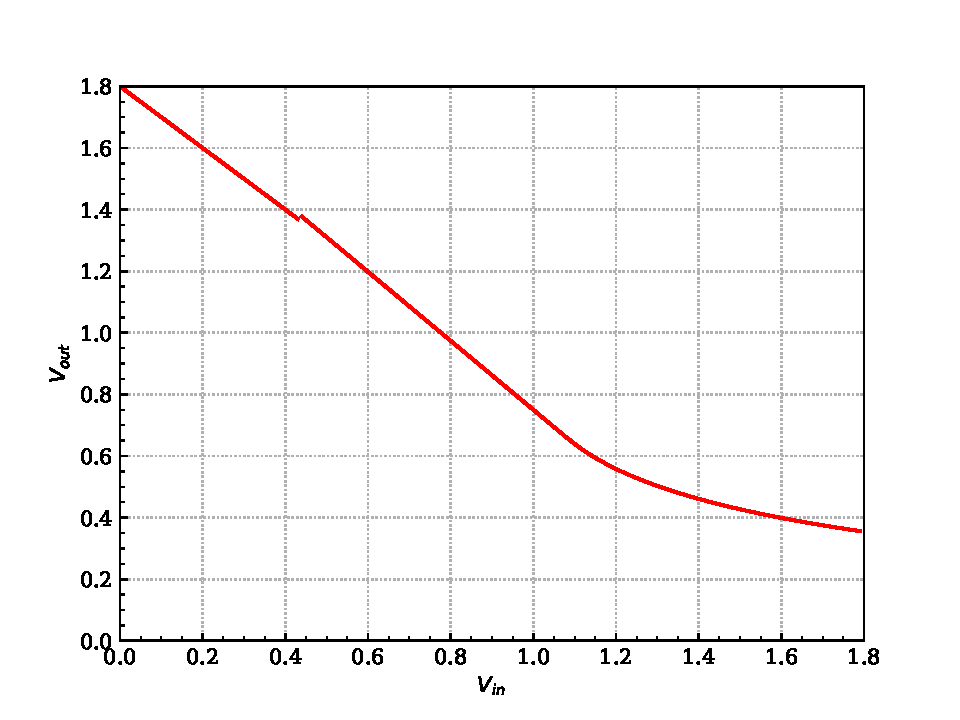
\includegraphics[width=.9\linewidth]{img/q7/a/cir1-vout-cal.pdf}
\end{center}

\item Simulated V\textsubscript{out}-V\textsubscript{in} relation using LTSpice

\begin{center}
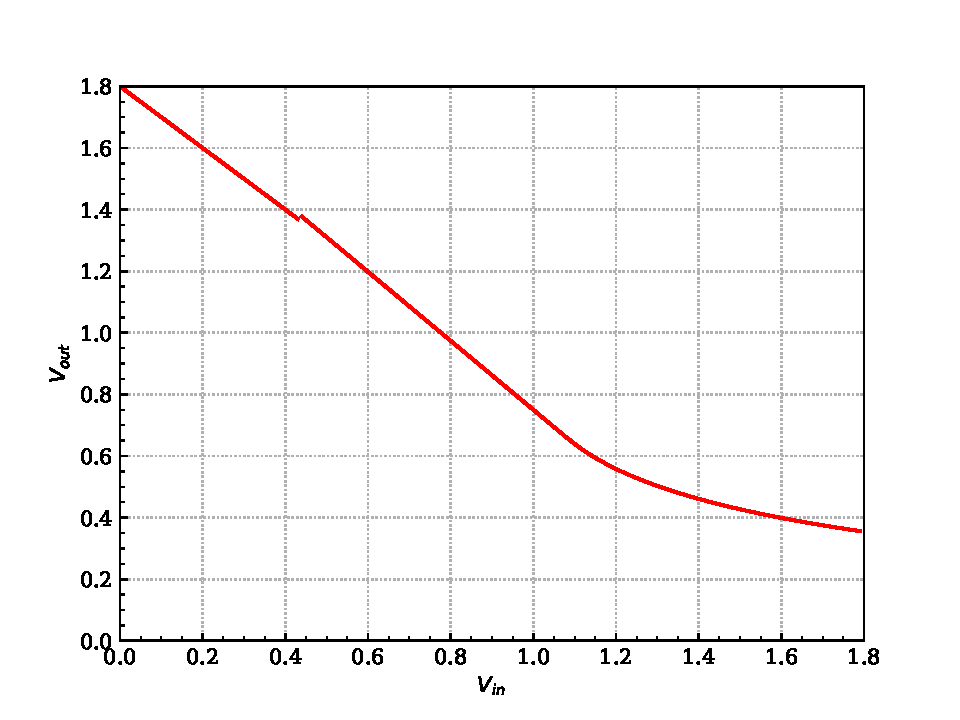
\includegraphics[width=.9\linewidth]{img/q7/a/cir1-vout-cal.pdf}
\end{center}

\item Maximum small-signal gain
For maximum small-signal gain:
\begin{equation*}
\begin{align}
max(|A_{V}|) &= max(|\frac{\partial{V_{out}}}{\partial{V_{in}}}|) \\
\\
V_{in} &\approx 0.69 V
\end{align}
\end{equation*}
\begin{center}
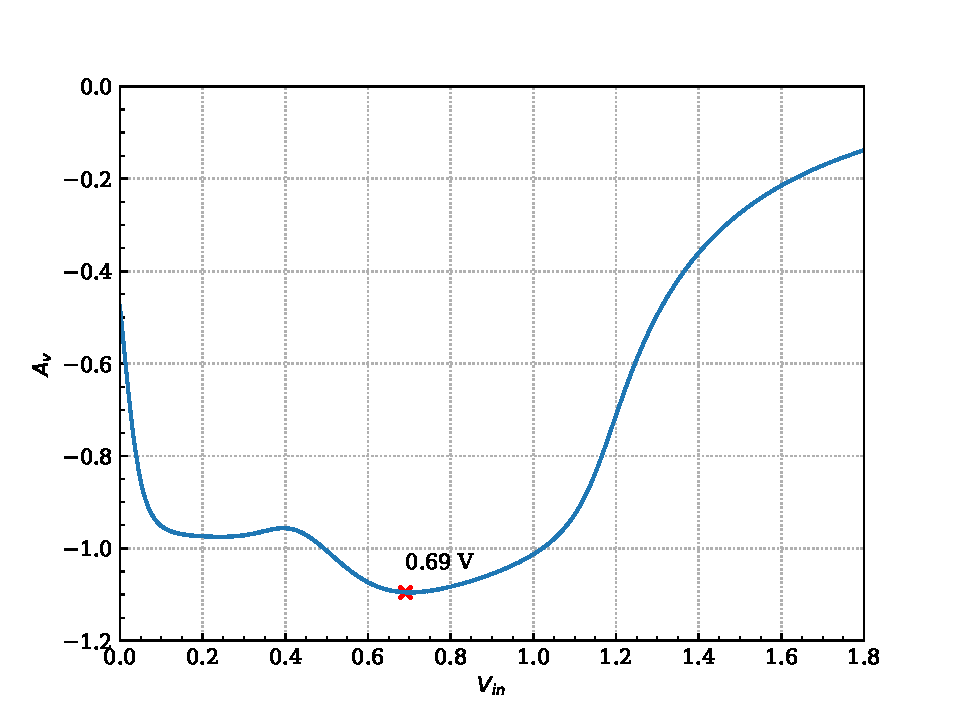
\includegraphics[width=.9\linewidth]{img/q7/c/cir1-d-vout.pdf}
\end{center}
\item 

\item 
\end{enumerate}
\end{document}
